\documentclass[a4paper,12pt]{article}

% Path to exercise sources
\newcommand{\path}{../}

% Preamble packages and inputs

\usepackage{\path/packages/boites}
\usepackage{\path/packages/courslatex}
\usepackage{\path/packages/fontesEval}
% Nécessaire si on utilise l'inclusion des exos à partir des fichiers

\input{\path/preambules/print_exo.tex}


% Tcolorbox settings
\tcbset{
    width=0.7\textwidth,
    height=1.5cm,
    colframe=black,
    colback=white,
    arc=10pt,
    valign=bottom,
}
% Document start
\begin{document}
\begin{center}
	Géométrie 1 -- à rendre pour le jeudi 13.3.25
\begin{tcolorbox}
	{\bfseries Seulement le prénom~:}~\makebox[7.5cm]{\hrulefill}\end{tcolorbox}
\end{center}

\begin{center}
	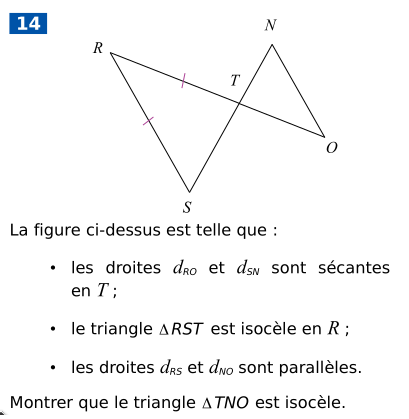
\includegraphics[scale=0.5]{../pics/ex14}
\framebox(550,450){}
\end{center}

% End of document
\end{document}

